%! suppress = EscapeHashOutsideCommand
%! Author = Theodore Capinski
%! Date = 3/5/2024

% Preamble
\documentclass[11pt]{article}
\let\oldsection\section
\renewcommand\section{\clearpage\oldsection}
\setcounter{section}{-1}
\counterwithin{figure}{section}

% Packages
\usepackage{amsmath}
\usepackage{hyperref}
\usepackage{graphicx}
\usepackage{tikz}
\usepackage{indentfirst}
\usepackage{circuitikz}

%%%%%%%%%%%%%%%%%%%%%%%%%%%%%%%%%%%%%%%%%%%%%%%%%%%%%%%%%%%%%%%%%%%%%%
% LaTeX Overlay Generator - Annotated Figures v0.0.1
% Created with http://ff.cx/latex-overlay-generator/
%%%%%%%%%%%%%%%%%%%%%%%%%%%%%%%%%%%%%%%%%%%%%%%%%%%%%%%%%%%%%%%%%%%%%%
%\annotatedFigureBoxCustom{bottom-left}{top-right}{label}{label-position}{box-color}{label-color}{border-color}{text-color}
\newcommand*\annotatedFigureBoxCustom[8]{\draw[#5,thick,rounded corners] (#1) rectangle (#2);\node at (#4) [fill=#6,thick,shape=circle,draw=#7,inner sep=2pt,font=\sffamily,text=#8] {\textbf{#3}};}
%\annotatedFigureBox{bottom-left}{top-right}{label}{label-position}
\newcommand*\annotatedFigureBox[4]{\annotatedFigureBoxCustom{#1}{#2}{#3}{#4}{white}{white}{black}{black}}
\newcommand*\annotatedFigureText[4]{\node[draw=none, anchor=south west, text=#2, inner sep=0, text width=#3\linewidth,font=\sffamily] at (#1){#4};}
\newenvironment {annotatedFigure}[1]{\centering\begin{tikzpicture}
                                                   \node[anchor=south west,inner sep=0] (image) at (0,0) { #1};\begin{scope}[x={(image.south east)},y={(image.north west)}]}{\end{scope}\end{tikzpicture}}
%%%%%%%%%%%%%%%%%%%%%%%%%%%%%%%%%%%%%%%%%%%%%%%%%%%%%%%%%%%%%%%%%%%%%%

\newcommand{\todo}[1]{\textcolor{red}{TODO: #1}\PackageWarning{TODO:}{#1!}}

\title{Physics 5BL Lab Report EM1}
\author{T.~Capinski \and A.~Patel}

% Document
\begin{document}
    \maketitle
    \tableofcontents

    \section*{Introduction}\label{sec:introduction}
    \addcontentsline{toc}{section}{Introduction}

    This report will cover the Ohm's Law lab.
    We will be measuring resistance, voltage with resistors in series, and ohmic and non-ohmic behaviour.
    We will also be discussing Kirchhoff's Laws.

    Ohm's law states that the current through a conductor between two points is directly proportional to the voltage across the two points.
    This relationship is represented by the equation
    \begin{equation}\label{eq:ohm_equation}
        V = I \cdot R
    \end{equation}
    where $V$ is the voltage, $I$ is the current, and $R$ is the resistance.
    Such a relationship is linear and is known as ohmic behaviour.
    To find the resistance of a material, we can use the equation
    \begin{equation}\label{eq:resistance_equation}
        R = \frac{V}{I}
    \end{equation}

    As covered in the report overview, resistors in series can be summed, such as
    \begin{equation}\label{eq:resistors_in_series}
        R_{\text{total}} = R_1 + R_2 + \ldots
    \end{equation}
    and when in parallel, the reciprocals of the resistances can be summed, such as
    \begin{equation}\label{eq:resistors_in_parallel}
        \frac{1}{R_{\text{total}}} = \frac{1}{R_1} + \frac{1}{R_2} + \ldots
    \end{equation}

    Finally, Kirchhoff's Laws are used to analyze complex circuits.
    The first law states that the sum of currents entering a junction is equal to the sum of currents leaving the junction.
    The second law states that the sum of the voltage drops around a closed loop is equal to the voltage supplied.
    \begin{equation}\label{eq:kirchhoff}
        \sum V = \sum I R
    \end{equation}
    \begin{equation}\label{eq:kirchhoff2}
        \sum I = 0
    \end{equation}

    To determine if our measured values are accurate, we will compare them to the theoretical values using an agreement test.
    The agreement test is defined as
    \begin{equation}\label{eq:agreement_test}
        |R_{\text{mea}} - R_{\exp}| \le 2 \sqrt{\alpha^2_{\text{mea}} -
        \alpha^2_{\exp} }
    \end{equation}


    \section{Measuring Resistance}\label{sec:measuring-resistance}


    \subsection{Methods}\label{subsec:resistance_methods}

    This lab will use a digital multimeter (DMM) to measure the resistance across a 1 $\Omega$ resistor.
    The procedure was fairly simple.
    The DMM was set to measure resistance, and the banana cables were connected to the resistor.
    This can be seen in Figure~\ref{fig:resistance_setup}.

    \begin{figure}[h]
        \begin{annotatedFigure}
        {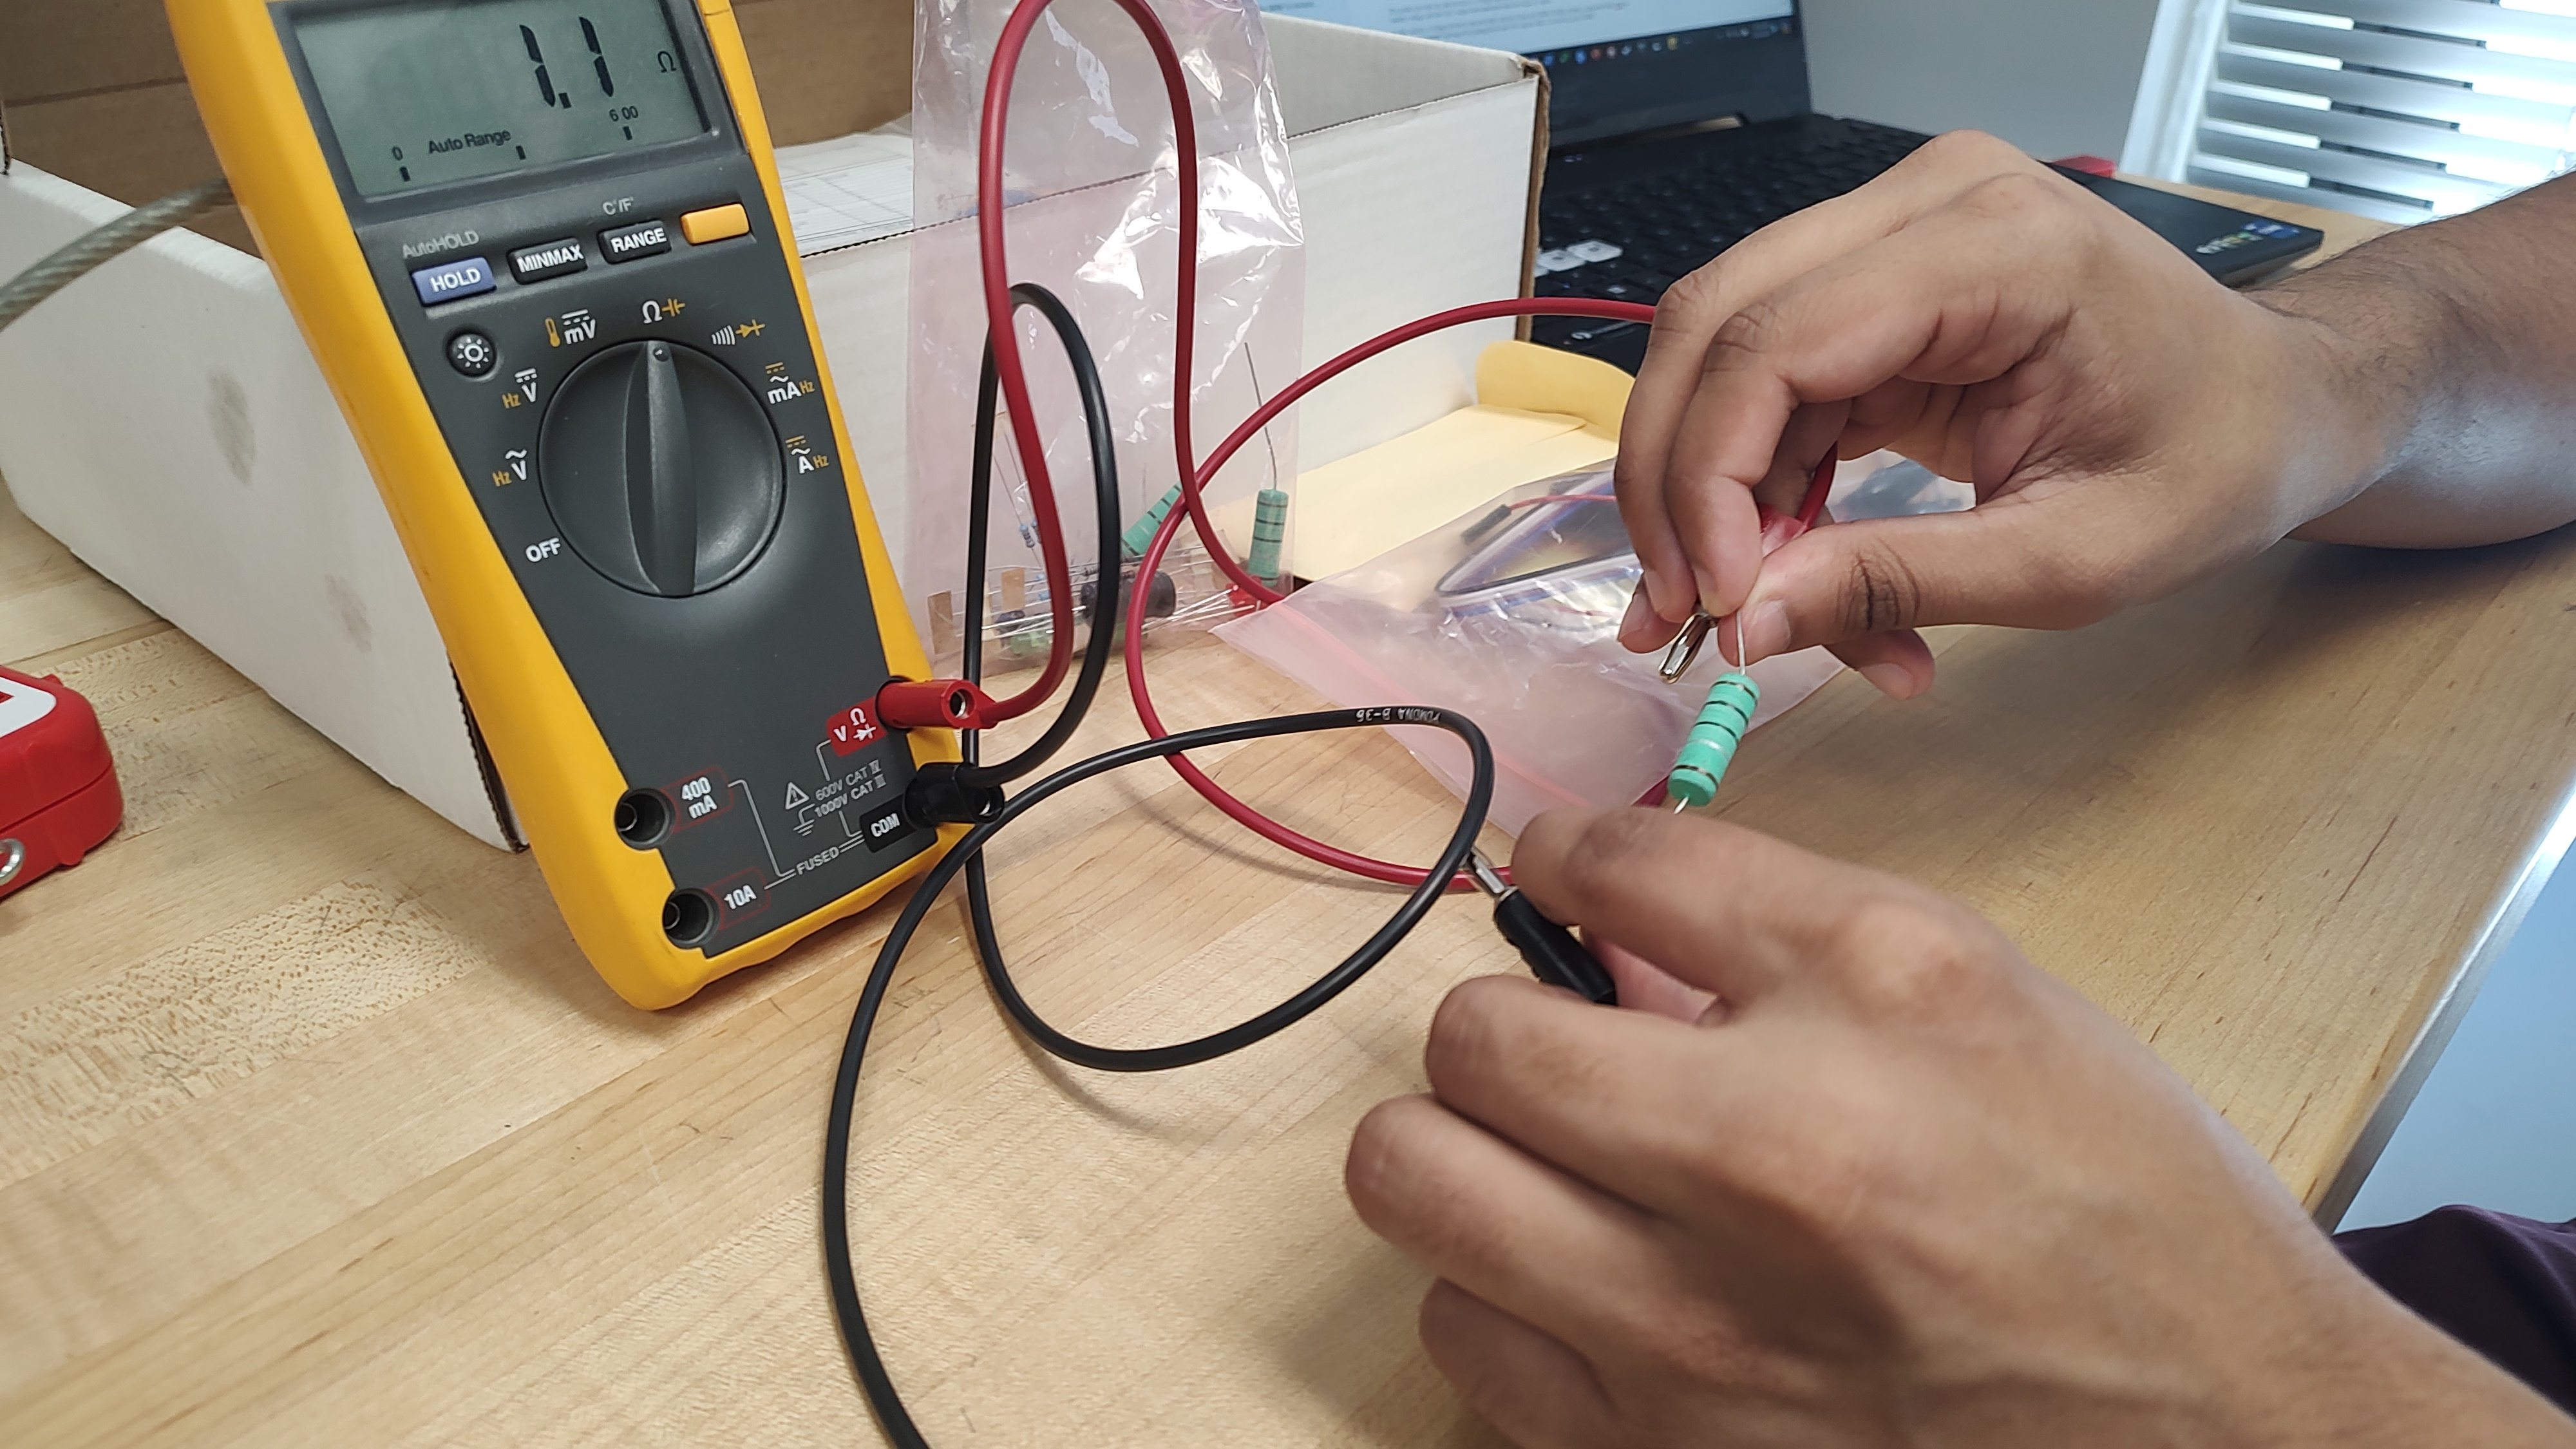
\includegraphics[width=1.0\linewidth]{resources/images/part0_setup}}
            \annotatedFigureBox{0.138,0.3873}{0.348,0.9773}{A}{0.138,0.3873}%bl
            \annotatedFigureBox{0.606,0.424}{0.736,0.5378}{B}{0.606,0.424}%bl
            \annotatedFigureBox{0.586,0.5419}{0.716,0.6907}{C}{0.586,0.5419}%bl
            \annotatedFigureBox{0.54,0.2497}{0.67,0.3983}{D}{0.54,0.2497}%bl
        \end{annotatedFigure}

        \caption{The DMM (A) measures the resistance across a 1 $\Omega$ resistor (B) via banana cables (C) and (D).}
        \label{fig:resistance_setup}
    \end{figure}

    \subsection{Analysis and Conclusion}\label{subsec:resistance_analysis}

    The resistance was measured to be 1.1 $\Omega$.
    The nominal value for the resistance was $1 \pm 1\%~\Omega$.
    The agreement test, from Equation~\ref{eq:agreement_test}, shows that the measured value is within the expected range.
    \begin{e}
        \begin{align*}
            |1.1 - 1| &\le 2 \sqrt{0.001^2 - 0.01^2} \\
            0.1 &\le 2 \sqrt{0} \\
            0.1 &\le 0
        \end{align*}
    \end{e}
    \todo{fix the above equation}

    This considers the error in the measurement and the error in the expected value.
    The use of a DMM makes human error virtually nonexistent.
    In conclusion, the measured resistance is within the expected range, and the DMM is a reliable tool for measuring resistance.

    \section{Voltage With Resistors in Series}\label{sec:voltage}

    \subsection{Methods}\label{subsec:voltage_methods}

    \begin{figure}[h]
        \begin{center}
            \begin{circuitikz}[american]
                \draw (0,0) to[battery1=$V_1$, inverted] ++(6,0)
                -- ++(0,-3)
                to[R=$R_1$] ++(-3,0)
                to[R=$R_2$, *-*] ++(-3,0)
                -- ++(0,3);
            \end{circuitikz}
        \end{center}
        \caption {Abstract circuit configuration for measuring current. $R_2$ is the 1 $\Omega$ resistor which it is measured across.}
        \label{fig:current_setup}
    \end{figure}

    \subsection{Analysis}\label{subsec:voltage_analysis}

    \subsection{Conclusion}\label{subsec:voltage_conclusion}

    \section{Ohmic and Non-Ohmic Behaviour}\label{sec:ohmic}

    \subsection{Methods}\label{subsec:ohmic_methods}

    \begin{figure}[h]
        \begin{annotatedFigure}
        {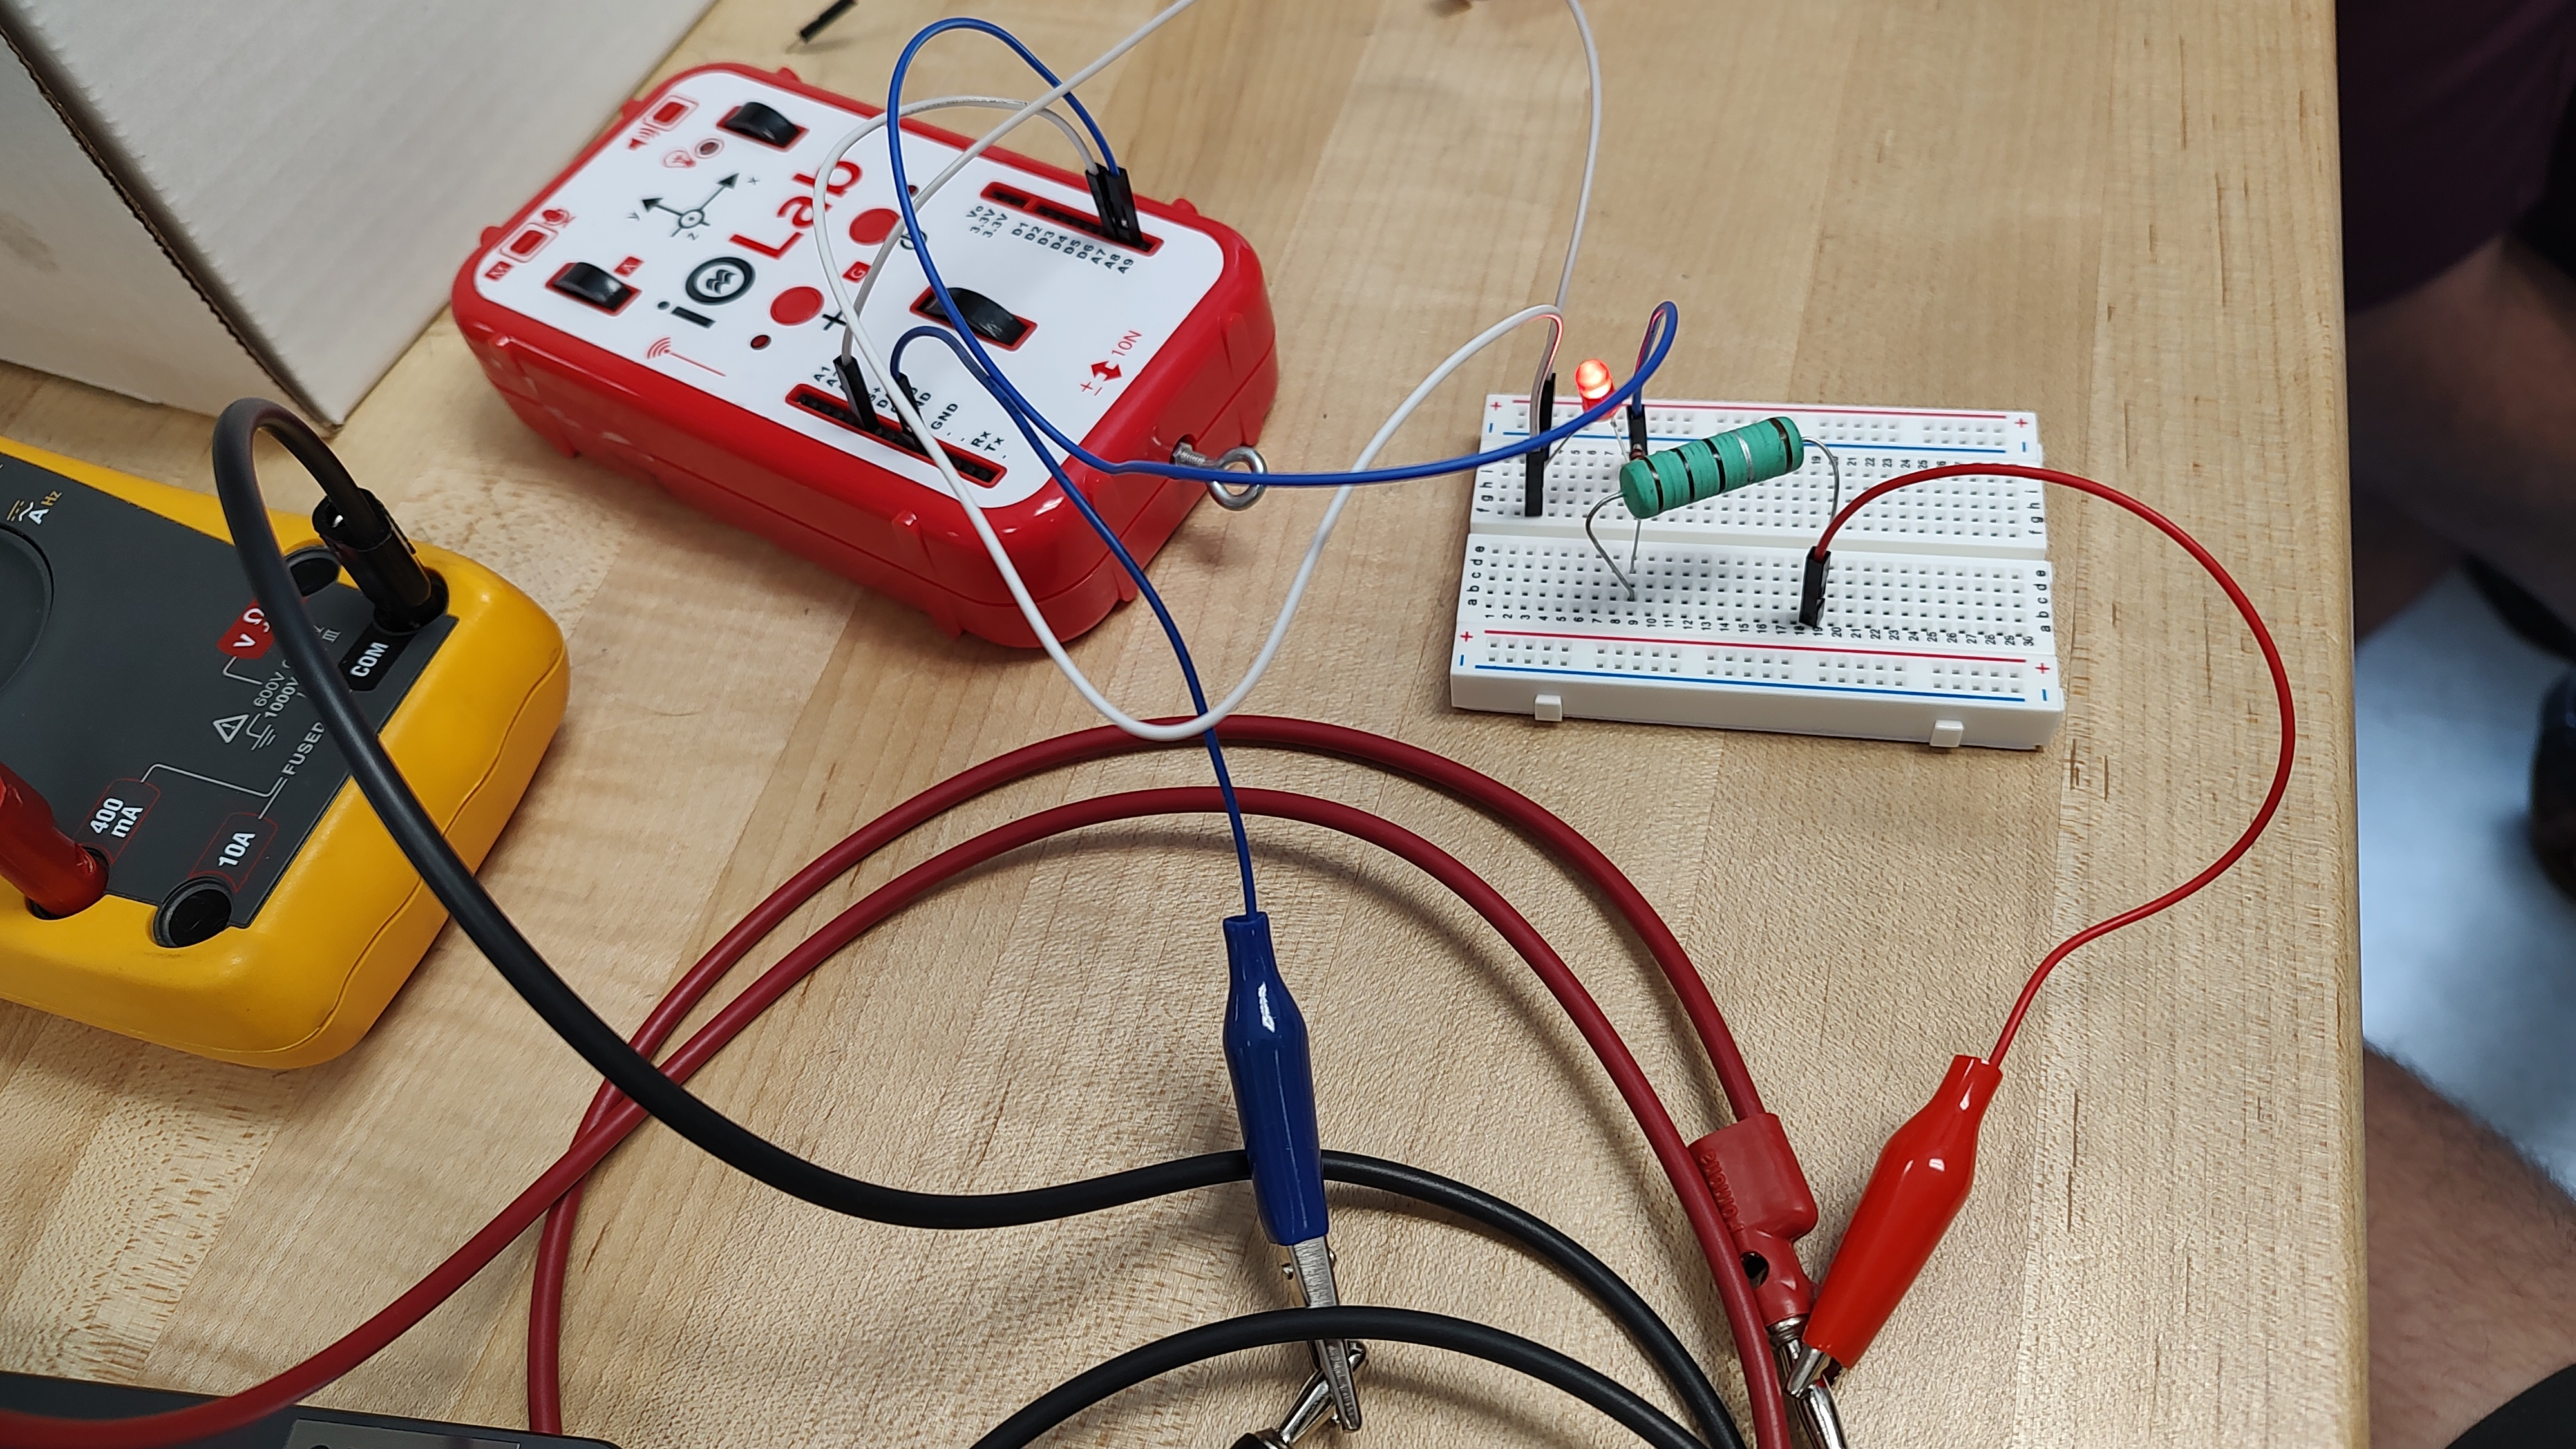
\includegraphics[width=1.0\linewidth]{resources/images/part2_setup}}
            \annotatedFigureBox{0.196,0.6112}{0.483,0.946}{A}{0.196,0.6112}%bl
            \annotatedFigureBox{0.642,0.6217}{0.7352,0.7262}{B}{0.642,0.6217}%bl
            \annotatedFigureBox{0.585,0.6934}{0.639,0.7834}{C}{0.585,0.6934}%bl
            \annotatedFigureBox{0.011,0.3155}{0.177,0.6714}{D}{0.011,0.3155}%bl
        \end{annotatedFigure}
        \caption{The IOLab (A) provides a voltage that runs through the breadboard. On the board a 1 $\Omega$ resistor (B) and an LED (C) are connected. The ground is connected via banana cables that go through the DMM (D).}
        \label{fig:ohmic_setup}
    \end{figure}

    To verify Ohm's Law, we set up a circuit with a 1 $\Omega$ resistor and an LED.
    The IOLab was used to provide a voltage to the circuit.
    The DMM was used to measure the voltage across the resistor.
    This can be seen in Figure~\ref{fig:ohmic_setup}.
    The IOLab was set to provide a voltage ranging from 1 V to 3.3 V.

    First, we measured Ohmic behaviour.
    The DMM was set to measure voltage, and the banana cables were connected to the resistor.
    We recorded the voltage across the resistor as the voltage was increased.
    This resulted in the following data:

    \begin{figure}[h]
        \centering
        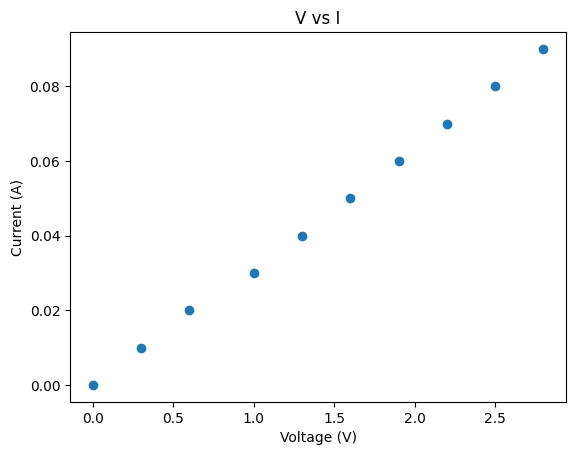
\includegraphics[width=1.0\textwidth]{resources/images/em1_2a_VvsI}
        \caption{Voltage and current data for the ohmic behaviour experiment.}
        \label{fig:ohmic_data}
    \end{figure}

    The data shows a linear relationship between the voltage and the current, as expected.

    Next, we measured non-ohmic behaviour.
    The LED was connected in series with a 1 k$\Omega$ resistor.
    We recorded the voltage across the LED as the DAC voltage was increased.
    This resulted in the following data:
    \begin{figure}[h!]
        \begin{align*}
            \begin{array}{|c|c|}
                \hline
                \text{Voltage (V)} & \text{Current (A)} \\
                \hline
                0.0 & 0.0 \\
                0.3 & 0.01 \\
                0.6 & 0.02 \\
                1.0 & 0.03 \\
                1.3 & 0.04 \\
                1.6 & 0.05 \\
                1.9 & 0.06 \\
                2.2 & 0.07 \\
                2.5 & 0.08 \\
                2.8 & 0.09 \\
                3.3 & 0.1 \\
                \hline
            \end{array}
        \end{align*}
        \caption{Voltage and current data for the non-ohmic behaviour experiment.}
        \label{fig:non_ohmic_data}
    \end{figure}
    \todo{graph the non-ohmic data}

    \subsection{Analysis}\label{subsec:ohmic_analysis}

    \subsection{Conclusion}\label{subsec:ohmic_conclusion}

    \section{Kirchhoff's Laws}\label{sec:kirchoff}

    \subsection{Methods}\label{subsec:kirchoff_methods}

    \begin{figure}[h]
        \begin{center}
            \begin{circuitikz}[american]
                \draw (0,0) to[battery1=$V_1$] ++(0,3)
                to[R=$R_1$] ++(3,0) coordinate(P1)
                to[R=$R_3$, -*] ++(0,-3)
                node[above right] {$A$}
                -- (0,0);
                \draw (P1) to[R=$R_2$] ++(3,0)
                to[battery1, l=$V_2$] ++(0,-3) -- ++(-3,0);
            \end{circuitikz}
        \end{center}
        \caption {Abstract circuit configuration for Kirchhoff's Laws experiment.}
        \label{fig:kirchoff_setup}
    \end{figure}

    For this experiment, we set up a circuit with three resistors.
    The goal was the measure the current before and after Junction $A$.
    To measure the current, we placed 1 $\Omega$ resistors before and after the junction.
    This can be seen in Figure~\ref{fig:kirchoff_setup}.
    We then used the DMM to measure the voltage across the resistors.
    The 1 $\Omega$ resistors added a negligible amount of resistance to the circuit, allowing them to act as ammeters.

    \todo{Add the kirchhoff setup figure}

    \subsection{Analysis}\label{subsec:kirchoff_analysis}

    Given figure~\ref{fig:kirchoff_setup}, we can use Kirchhoff's Laws to analyze the expected currents in the circuit.
    Taking $I_1$ as the initial current from the DAC, $I_2$ as the current after the batteries, and $I_3$ as the current after the resistor $R_3$, we can use the following equations:
    \begin{align*}
        Loop~1: V_1 - I_1 R_1 - I_2 R_2 &= 0 \\
        Loop~2: V_2 - I_2 R_2 - I_3 R_3 &= 0 \\
        Junction~A: I_3 - I_2 - I_1 &= 0
    \end{align*}
    \todo{Explain the sign of each term?}
    These equations give:
    \begin{align*}
        I_1 &= \frac{V_1(R_2 + R_3) - V_2 R_3}{R_1 R_2 + R_2 R_3 + R_1 R_3} \\
        I_2 &= \frac{V_2(R_1 + R_3) - V_1 R_3}{R_1 R_2 + R_2 R_3 + R_1 R_3} \\
        I_3 &= \frac{V_1 R_2 + V_2 R_1}{R_1 R_2 + R_2 R_3 + R_1 R_3}
    \end{align*}
    For this experiment, we used:
    \begin{align*}
        V_1 &= 3.3 \pm 0.1 \text{ V} \\
        V_2 &= 4.5 \pm 0.1 \text{ V} \\
        R_1 &= 4.7k \pm 0.1k \text{ $\Omega$} \\
        R_2 &= 10k \pm 0.1k \text{ $\Omega$} \\
        R_1 &= 4.7k \pm 0.1k \text{ $\Omega$}
    \end{align*}
    which results in expected values for the currents of approximately:
%    ['I1: 0.236 mA', 'I2: 0.231 mA', 'I3: 0.466 mA']
    \begin{align*}
        I_{1exp} &= 0.3 \pm 0.1 \text{ A} \\
        I_{2exp} &= 0.3 \pm 0.1 \text{ A} \\
        I_{3exp} &= 0.6 \pm 0.1 \text{ A}
    \end{align*}
    \todo{Propogate the error}

    With the DMM, we measured the currents to be:
    \begin{align*}
        I_{1mea} &= 0.236 \pm 0.001 \text{ A} \\
        I_{2mea} &= 0.231 \pm 0.001 \text{ A} \\
        I_{3mea} &= 0.466 \pm 0.001 \text{ A}
    \end{}
    \todo{Actually use the DMM to measure the currents}

    The agreement test, from Equation~\ref{eq:agreement_test}, shows that the measured values are within the expected range.
    \begin{e}
        \begin{align*}
            |0.236 - 0.3| &\le 2 \sqrt{0.001^2 - 0.1^2} \\
            0.064 &\le 2 \sqrt{0} \\
            0.064 &\le 0
        \end{align*}
    \end{e}
    \todo{Fix the above equation (filled in by copilot)}

    \subsection{Conclusion}\label{subsec:kirchoff_conclusion}

    \todo{Explain the results of the agreement test}
    \todo{Consider sources of error}
    etc\ldots

\end{document}